\documentclass[12pt,a4paper]{article}

% ─── Page Layout ───────────────────────────────────────────────────────────────
\usepackage[a4paper, margin=0.8in, headheight=14pt]{geometry}

% ─── Fonts (XeLaTeX) ───────────────────────────────────────────────────────────
\usepackage{fontspec}
\usepackage{unicode-math}
\setmainfont{TeX Gyre Pagella}
\setmonofont[Scale=0.88]{TeX Gyre Cursor}
\setmathfont{Latin Modern Math}

% ─── Packages ──────────────────────────────────────────────────────────────────
\usepackage{xcolor}
\usepackage{colortbl}
\usepackage{titlesec}
\usepackage{enumitem}
\usepackage{tabularx}
\usepackage{booktabs}
\usepackage{array}
\usepackage{amsmath}
\usepackage{tikz}
\usetikzlibrary{shapes.geometric, arrows.meta, positioning, calc, fit, decorations.pathreplacing, decorations.pathmorphing}
\usepackage{tcolorbox}
\tcbuselibrary{skins, breakable}
\usepackage{hyperref}
\usepackage{fancyhdr}
\usepackage{graphicx}
\usepackage{microtype}
\hyphenpenalty=10000
\exhyphenpenalty=10000
\sloppy
\usepackage{caption}
\usepackage{setspace}
\usepackage{multirow}
\usepackage{tocloft}

% ─── Q&A helper ────────────────────────────────────────────────────────────────
\newcommand{\Q}[1]{\textbf{#1}\par\noindent\ignorespaces}

% ─── Colour Palette ────────────────────────────────────────────────────────────
\definecolor{myred}{RGB}{196,30,58}
\definecolor{mydark}{RGB}{30,30,50}
\definecolor{mygreen}{RGB}{14,120,80}
\definecolor{myteal}{RGB}{0,130,140}
\definecolor{myamber}{RGB}{180,100,0}
\definecolor{mypurple}{RGB}{100,30,160}
\definecolor{mygray}{RGB}{246,247,249}
\definecolor{mgframe}{RGB}{180,185,200}
\definecolor{watermark}{RGB}{145,150,170}
\definecolor{hdrred}{RGB}{250,232,235}
\definecolor{hdrgreen}{RGB}{220,244,233}
\definecolor{hdrteal}{RGB}{220,242,244}
\definecolor{hdramber}{RGB}{253,242,215}
\definecolor{hdrpurple}{RGB}{238,228,255}
\definecolor{hdrgray}{RGB}{238,240,245}
\definecolor{rowalt}{RGB}{250,251,253}

% ─── Section Formatting ────────────────────────────────────────────────────────
\titleformat{\section}
  {\large\bfseries\color{myred}}{\thesection.}{0.5em}{}
  [\vspace{1pt}{\color{myred}\rule{\linewidth}{0.8pt}}]
\titleformat{\subsection}
  {\normalsize\bfseries\color{myteal}}{\thesubsection}{0.5em}{}
\titlespacing*{\section}{0pt}{18pt}{7pt}
\titlespacing*{\subsection}{0pt}{11pt}{4pt}

% ─── Paragraph ─────────────────────────────────────────────────────────────────
\setlength{\parindent}{0pt}
\setlength{\parskip}{4pt}

% ─── TOC Styling ───────────────────────────────────────────────────────────────
\renewcommand{\cfttoctitlefont}{\large\bfseries\color{myred}}
\renewcommand{\cftaftertoctitle}{\par\noindent{\color{myred}\rule{\linewidth}{0.8pt}}}
\setlength{\cftbeforetoctitleskip}{0pt}
\setlength{\cftaftertoctitleskip}{6pt}
\renewcommand{\cftsecfont}{\normalsize\bfseries\color{mydark}}
\renewcommand{\cftsecpagefont}{\normalsize\bfseries\color{mydark}}
\renewcommand{\cftsecleader}{\cftdotfill{\cftdotsep}}
\setlength{\cftbeforesecskip}{7pt}
\renewcommand{\cftsubsecfont}{\small\color{mydark}}
\renewcommand{\cftsubsecpagefont}{\small\color{mydark}}
\setlength{\cftbeforesubsecskip}{3pt}
\setlength{\cftsubsecindent}{1.4em}

% ─── Table helpers ─────────────────────────────────────────────────────────────
\renewcommand{\arraystretch}{1.45}
\setlength{\tabcolsep}{6pt}
\arrayrulecolor{mydark}
\newcolumntype{B}[1]{>{\small\bfseries\raggedright\arraybackslash}m{#1}}
\newcolumntype{Y}{>{\small\raggedright\arraybackslash}X}
\renewcommand{\tabularxcolumn}[1]{m{#1}}

% ─── Header / Footer ───────────────────────────────────────────────────────────
\pagestyle{fancy}
\fancyhf{}
\fancyhead[L]{\small\color{myred}\textbf{PE-EC603A}\;\color{mydark}--- Introduction to MEMS}
\fancyhead[R]{\small\color{myteal}\textbf{Module 4 Notes}}
\fancyfoot[C]{\small\color{mydark}\thepage}
\fancyfoot[R]{\small\color{watermark}\textit{\copyright\ Biraj}}
\renewcommand{\headrulewidth}{0.5pt}
\renewcommand{\footrulewidth}{0.3pt}

% ─── Hyperref ──────────────────────────────────────────────────────────────────
\hypersetup{
  colorlinks=true, linkcolor=myteal, urlcolor=myteal,
  pdfauthor={Biraj Sarkar},
  pdftitle={PE-EC603A --- Module 4 Notes}
}

% ─── tcolorbox styles ──────────────────────────────────────────────────────────
\tcbset{
  tikzbox/.style={
    colback=mygray, colframe=mgframe, boxrule=0.6pt, arc=4pt,
    left=8pt, right=8pt, top=6pt, bottom=6pt,
    colbacktitle=mgframe, coltitle=mydark,
    fonttitle=\small\bfseries
  },
  defbox/.style={
    colback=hdrgreen, colframe=mygreen, boxrule=0.8pt, arc=4pt,
    left=9pt, right=9pt, top=6pt, bottom=6pt,
    colbacktitle=mygreen, coltitle=white,
    fonttitle=\small\bfseries
  },
  formulabox/.style={
    colback=hdrteal, colframe=myteal, boxrule=0.8pt, arc=4pt,
    left=9pt, right=9pt, top=7pt, bottom=7pt,
    colbacktitle=myteal, coltitle=white,
    fonttitle=\small\bfseries
  },
  examplebox/.style={
    colback=hdramber, colframe=myamber, boxrule=0.8pt, arc=4pt,
    left=9pt, right=9pt, top=6pt, bottom=6pt,
    colbacktitle=myamber, coltitle=white,
    fonttitle=\small\bfseries
  },
  masonbox/.style={
    colback=hdrpurple, colframe=mypurple, boxrule=0.8pt, arc=4pt,
    left=9pt, right=9pt, top=6pt, bottom=6pt,
    colbacktitle=mypurple, coltitle=white,
    fonttitle=\small\bfseries
  },
  exambox/.style={
    colback=hdrpurple, colframe=mypurple, boxrule=1pt, arc=5pt,
    left=10pt, right=10pt, top=8pt, bottom=8pt,
    colbacktitle=mypurple, coltitle=white,
    fonttitle=\bfseries,
    breakable, title after break={\textbf{Frequently Asked / Viva Questions (contd.)}}}
}
% Make all boxes breakable across pages
\tcbset{breakable}

% ─── TikZ styles ───────────────────────────────────────────────────────────────
\tikzset{
  block/.style={rectangle, draw=myteal, fill=hdrteal,
    text width=2.4cm, align=center, minimum height=0.95cm,
    font=\small, rounded corners=3pt, line width=0.7pt},
  redblock/.style={rectangle, draw=myred, fill=hdrred,
    text width=2.4cm, align=center, minimum height=0.95cm,
    font=\small, rounded corners=3pt, line width=0.7pt},
  netnode/.style={rectangle, draw=myteal, fill=hdrteal,
    text width=1.5cm, align=center, minimum height=0.8cm,
    font=\small, rounded corners=3pt, line width=0.7pt},
  sumjunc/.style={circle, draw=myamber, fill=hdramber,
    minimum size=0.62cm, font=\small, line width=0.8pt},
  snode/.style={circle, draw=mypurple, fill=hdrpurple,
    minimum size=0.55cm, font=\footnotesize, line width=0.7pt},
  arrow/.style={-Stealth, thick, color=mydark},
  redarrow/.style={-Stealth, thick, color=myred},
  line/.style={thick, color=mydark}
}

% ═══════════════════════════════════════════════════════════════════════════════
\begin{document}
% ═══════════════════════════════════════════════════════════════════════════════

\begin{center}
  {\LARGE\bfseries\color{myred} PE-EC603A --- Introduction to MEMS}\\[5pt]
  {\normalsize\color{mydark} Semester VI \quad$\bullet$\quad 3L:0T:0P \quad$\bullet$\quad 3 Credits}\\[3pt]
  {\normalsize\color{myteal}\textbf{Module 4 Exam Notes: Bulk Micromachining \& Mechanics}}\\[3pt]
  {\small\color{mydark} CGEC \;$|$\; B.Tech ECE (2023--27) \;$|$\; \textit{Biraj Sarkar}}
\end{center}
\vspace{2pt}
\noindent{\color{myred}\rule{\linewidth}{1.5pt}}
\vspace{2pt}

\hypersetup{linkcolor=mydark}
\tableofcontents
\hypersetup{linkcolor=myteal}
\newpage

% ===============================================================================
\section{Bulk Micromachining \& Wafer Bonding}
% ===============================================================================

Bulk micromachining fabricates micro-structures directly inside the substrate by selectively etching away deep portions of the silicon wafer.

\subsection{Wet Isotropic vs. Anisotropic Etching}
\begin{itemize}[leftmargin=*, itemsep=4pt]
  \item \textbf{Isotropic Etching (HNA):}
    \begin{itemize}[leftmargin=*, itemsep=2.5pt]
      \item Uses a mixture of Hydrofluoric acid ($HF$), Nitric acid ($HNO_3$), and Acetic acid ($CH_3COOH$) --- known as \textbf{HNA}.
      \item \textbf{Mechanism:} Nitric acid oxidizes the silicon surface to form $SiO_2$, Hydrofluoric acid dissolves this oxide, and Acetic acid acts as a diluent to control reaction rate.
      \item Etches equally in all directions, leading to rounded cavities and mask undercutting.
    \end{itemize}
  \item \textbf{Anisotropic Etching (KOH / TMAH):}
    \begin{itemize}[leftmargin=*, itemsep=2.5pt]
      \item Uses Potassium Hydroxide (\textbf{KOH}) or Tetramethylammonium Hydroxide (\textbf{TMAH}).
      \item Etches along crystallographic planes. The etch rate is extremely slow on the $\{111\}$ plane compared to $\{100\}$ (selectivity up to $400:1$ for KOH).
      \item \textbf{Reason for Slow \{111\} Etch:} The $\{111\}$ plane has the highest atomic packing density, and surface atoms on $\{111\}$ present only a single dangling bond to the chemical solution (compared to two bonds on $\{100\}$), making it highly resistant to chemical attack.
      \item Results in precise V-grooves and pyramidal cavities with sidewalls sloped at an angle of $54.74^{\circ}$ relative to the $\{100\}$ surface.
    \end{itemize}
\end{itemize}

\subsection{Wafer Bonding Techniques}
Wafer bonding joins two substrates to form complex 3D structures or sealed packages:
\begin{enumerate}[leftmargin=*, label=\arabic*., itemsep=3.5pt]
  \item \textbf{Direct / Fusion Bonding:} Joins silicon to silicon. Silicon surfaces are polished, hydrated (creating silanol $Si-OH$ groups), pressed together, and annealed at high temperature ($>1000^{\circ}\text{C}$). The silanol groups polymerize to form strong covalent covalent bonds ($Si-O-Si$).
  \item \textbf{Anodic Bonding:} Joins silicon to sodium-rich glass (e.g., Pyrex 7740). The substrates are heated to $300^{\circ}\text{C}$--$450^{\circ}\text{C}$, and a high DC voltage ($400\text{ V}$--$1000\text{ V}$) is applied with glass as cathode. Sodium ions ($Na^+$) migrate away from the interface, creating a depletion region and strong electrostatic pull that initiates chemical bonding.
  \item \textbf{Eutectic Bonding:} Joins silicon to metal (e.g., Gold). They are heated to the eutectic temperature ($363^{\circ}\text{C}$ for $Au$--$Si$), forming a liquid alloy phase that solidifies to create a high-strength hermetic seal.
\end{enumerate}

% ===============================================================================
\section{Solid Mechanics at Microscale}
% ===============================================================================

Understanding mechanical deformation, stress, and strain is essential for designing MEMS suspensions.

\subsection{Stress, Strain, and Elastic Constants}
\begin{itemize}[leftmargin=*, itemsep=3.5pt]
  \item \textbf{Stress ($\sigma$):} Force per unit area ($\sigma = F / A$ in $\text{N/m}^2$ or $\text{Pa}$).
  \item \textbf{Strain ($\epsilon$):} Fractional elongation ($\epsilon = \Delta L / L$, dimensionless).
  \item \textbf{Hooke's Law:} States that within the elastic limit, stress ($\sigma$) is directly proportional to strain ($\epsilon$).
    \begin{itemize}[leftmargin=*, itemsep=2.5pt, topsep=0pt]
      \item \textbf{1D Formulation:} $\sigma = E \epsilon$ (where $E$ is Young's Modulus, a measure of stiffness).
      \item \textbf{Generalized 3D Formulation (Isotropic):} Relates 3D stresses and strains using Young's modulus ($E$) and Poisson's ratio ($\nu$):
        \begin{align}
          \epsilon_x &= \frac{1}{E} \left[ \sigma_x - \nu(\sigma_y + \sigma_z) \right] \\
          \epsilon_y &= \frac{1}{E} \left[ \sigma_y - \nu(\sigma_x + \sigma_z) \right] \\
          \epsilon_z &= \frac{1}{E} \left[ \sigma_z - \nu(\sigma_x + \sigma_y) \right]
        \end{align}
    \end{itemize}
  \item \textbf{Poisson's Ratio ($\nu$):} The ratio of transverse strain to axial strain under tensile load:
    \begin{equation}
      \nu = -\frac{\epsilon_{\text{transverse}}}{\epsilon_{\text{axial}}}
    \end{equation}
\end{itemize}

\subsection{Thermal Stress and Strain}
When a material with Coefficient of Thermal Expansion (\textbf{CTE}, $\alpha$) is heated by $\Delta T$, its free thermal strain is:
$$\epsilon_{\text{th}} = \alpha \Delta T$$
If the material is clamped at both ends, prevented from expanding, it experiences a thermal stress:
$$\sigma_{\text{th}} = -E \alpha \Delta T$$

This thermal stress is the primary driving mechanism in thermal actuators and a major source of thermal drift in capacitive sensors.

% ===============================================================================
\section{Cantilever Beam Deflection Derivation}
% ===============================================================================

Consider a rectangular cantilever beam of length $L$, width $w$, and thickness $h$ clamped at $x=0$, with a point force $F$ applied downward at the free end $x=L$.

\begin{tcolorbox}[tikzbox, title={Cantilever Beam Deflection Schematic}]
\centering
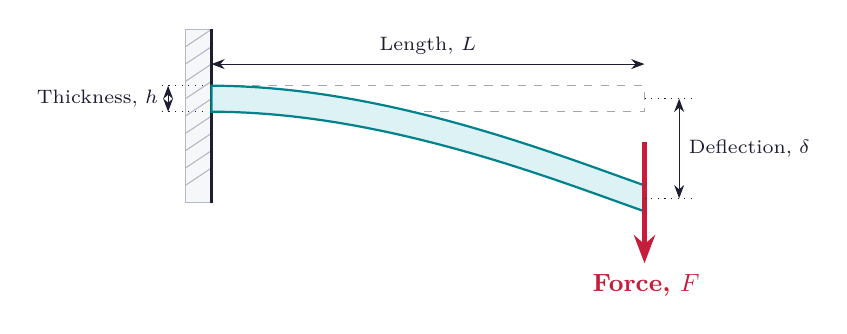
\begin{tikzpicture}[x=1.1cm, y=1.1cm, >=Stealth]
  % Clamped wall
  \draw[fill=mygray, draw=mgframe] (-0.3,-1.2) rectangle (0,0.8);
  \foreach \y in {-1.0,-0.8,...,0.6} {
    \draw[mgframe, thin] (-0.3,\y) -- (0,\y+0.2);
  }
  \draw[mydark, thick] (0,-1.2) -- (0,0.8);
  
  % Undeflected Beam
  \draw[mydark, dashed, opacity=0.4] (0,-0.15) rectangle (5.0,0.15);
  \draw[<->, mydark, thin] (0, 0.4) -- (5.0, 0.4) node[midway, above, font=\scriptsize] {Length, $L$};
  
  % Deflected Beam
  \draw[fill=hdrteal, draw=myteal, thick] 
    (0, 0.15) .. controls (2.0, 0.15) and (4.0, -0.65) .. (5.0, -1.0) -- 
    (5.0, -1.3) .. controls (4.0, -0.95) and (2.0, -0.15) .. (0, -0.15) -- cycle;
     
  % Force arrow
  \draw[redarrow, ultra thick] (5.0, -0.5) -- (5.0, -1.9) node[below, font=\small\bfseries\color{myred}] {Force, $F$};
  
  % Deflection dimension
  \draw[<->, mydark, thin] (5.4, 0) -- (5.4, -1.15) node[midway, right, font=\scriptsize] {Deflection, $\delta$};
  \draw[mydark, dotted] (5.0, 0) -- (5.6, 0);
  \draw[mydark, dotted] (5.0, -1.15) -- (5.6, -1.15);
  
  % Label thickness
  \draw[<->, mydark, thin] (-0.5, -0.15) -- (-0.5, 0.15) node[midway, left, font=\scriptsize] {Thickness, $h$};
  \draw[mydark, dotted] (-0.1, -0.15) -- (-0.6, -0.15);
  \draw[mydark, dotted] (-0.1, 0.15) -- (-0.6, 0.15);
\end{tikzpicture}
\end{tcolorbox}

The bending moment at any position $x$ along the beam length is:
$$M(x) = -F(L-x)$$
According to Euler-Bernoulli beam theory:
$$E I \frac{d^2 y}{dx^2} = M(x) = -F(L-x)$$
where $I$ is the rectangular moment of inertia:
$$I = \frac{w h^3}{12}$$
Integrate the differential equation once with respect to $x$:
$$E I \frac{dy}{dx} = -F \left(L x - \frac{x^2}{2}\right) + C_1$$
Applying the boundary condition at the clamped end ($x = 0$): $\frac{dy}{dx} = 0 \implies C_1 = 0$.
Integrate a second time:
$$E I y(x) = -F \left(L \frac{x^2}{2} - \frac{x^3}{6}\right) + C_2$$
Applying the boundary condition at $x = 0$: $y(0) = 0 \implies C_2 = 0$.
Thus, the deflection curve of the beam is:
$$y(x) = -\frac{F}{6 E I} (3 L x^2 - x^3)$$
The maximum deflection $\delta$ occurs at the free end $x = L$:
$$\delta = |y(L)| = \frac{F L^3}{3 E I}$$
Using the spring relation $F = k \delta$, the equivalent spring constant $k$ is:
$$k = \frac{3 E I}{L^3}$$
Substituting $I = \frac{w h^3}{12}$:
$$k = \frac{3 E}{L^3} \left(\frac{w h^3}{12}\right) = \frac{E w h^3}{4 L^3}$$

% ===============================================================================
\section{Coupled Electromechanical Pull-in Model}
% ===============================================================================

An electrostatic parallel-plate actuator experiences pull-in instability, where electrostatic forces overwhelm mechanical spring restoring forces.

\begin{tcolorbox}[tikzbox, title={Parallel-Plate Spring-Actuator Model}]
\centering
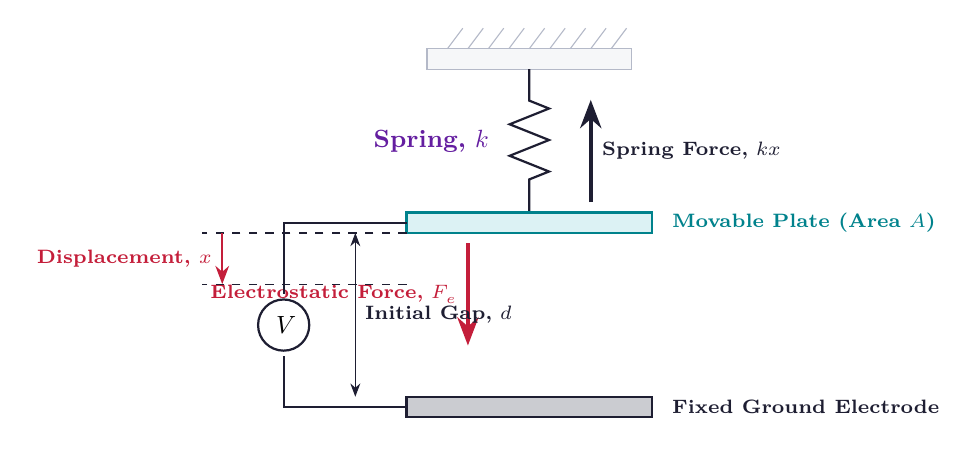
\begin{tikzpicture}[x=1.3cm, y=1.3cm, >=Stealth]
  % Rigid ceiling
  \draw[fill=mygray, draw=mgframe] (1.0,3.6) rectangle (3.0,3.8);
  \foreach \x in {1.2,1.4,...,2.8} {
    \draw[mgframe, thin] (\x,3.8) -- (\x+0.15,4.0);
  }
  
  % Spring
  \draw[mydark, thick, decoration={zigzag, pre length=4mm, post length=4mm, segment length=4mm, amplitude=2.5mm}, decorate] (2.0,3.6) -- (2.0,2.2);
  \node[anchor=east, font=\small\bfseries\color{mypurple}] at (1.7, 2.9) {Spring, $k$};
  
  % Spring Force Arrow
  \draw[arrow, ultra thick] (2.6, 2.3) -- (2.6, 3.3) node[midway, right, font=\scriptsize\bfseries\color{mygreen}] {Spring Force, $kx$};
  
  % Movable Plate
  \draw[fill=hdrteal, draw=myteal, thick] (0.8,2.0) rectangle (3.2,2.2);
  \node[anchor=west, font=\scriptsize\bfseries\color{myteal}] at (3.3,2.1) {Movable Plate (Area $A$)};
  
  % Fixed Ground Electrode
  \draw[fill=mygray!80!mydark, draw=mydark, thick] (0.8,0.2) rectangle (3.2,0.4);
  \node[anchor=west, font=\scriptsize\bfseries\color{mydark}] at (3.3,0.3) {Fixed Ground Electrode};
  
  % Electrostatic Force Arrow
  \draw[redarrow, ultra thick] (1.4, 1.9) -- (1.4, 0.9) node[midway, left, font=\scriptsize\bfseries\color{myred}] {Electrostatic Force, $F_e$};
  
  % Initial Gap Dimension Line
  \draw[<->, mydark, thin] (0.3, 0.4) -- (0.3, 2.0) node[midway, right, font=\scriptsize\bfseries] {Initial Gap, $d$};
  
  % Displacement Dashed Lines and Arrow
  \draw[dashed, mydark, thin] (0.8, 2.0) -- (-1.2, 2.0);
  \draw[dashed, mydark, thin] (0.8, 1.5) -- (-1.2, 1.5);
  \draw[->, myred, thick] (-1.0, 2.0) -- (-1.0, 1.5) node[midway, left, font=\scriptsize\bfseries] {Displacement, $x$};
  
  % Voltage source connection
  \draw[thick, mydark] (0.8,2.1) -- (-0.4,2.1) -- (-0.4,1.4);
  \draw[thick, mydark] (0.8,0.3) -- (-0.4,0.3) -- (-0.4,0.8);
  \draw[fill=white, draw=mydark, thick] (-0.4,1.1) circle (0.25);
  \node[font=\small\bfseries] at (-0.4,1.1) {$V$};
\end{tikzpicture}
\end{tcolorbox}

The force balance equation of the system at equilibrium is:
$$F_s = F_e \implies k x = \frac{1}{2} \frac{\epsilon A V^2}{(d-x)^2}$$
where $k$ is spring constant, $d$ is initial gap, and $x$ is displacement. Solve for $V^2$:
$$V^2 = \frac{2 k x (d-x)^2}{\epsilon A}$$
To find the limits of stable equilibrium, we find the maximum voltage that can be applied by taking the derivative with respect to $x$ and setting it to zero:
$$\frac{d(V^2)}{dx} = 0 \implies \frac{2k}{\epsilon A} \frac{d}{dx} \left[ x (d-x)^2 \right] = 0$$
$$\frac{d}{dx} \left( x d^2 - 2d x^2 + x^3 \right) = d^2 - 4d x + 3x^2 = 0$$
$$(d - 3x)(d - x) = 0$$
This yields two solutions: $x = d$ (unstable limit where gap is zero) and:
$$x_{\text{pi}} = \frac{d}{3}$$

\textbf{Conclusion 1:} The critical displacement at the pull-in point is exactly one-third of the initial gap.
Substitute $x_{\text{pi}} = d/3$ back into the voltage equation to find the critical \textbf{Pull-in Voltage} ($V_{\text{pi}}$):
$$V_{\text{pi}}^2 = \frac{2 k \left(\frac{d}{3}\right) \left(d - \frac{d}{3}\right)^2}{\epsilon A} = \frac{2 k \left(\frac{d}{3}\right) \left(\frac{2d}{3}\right)^2}{\epsilon A} = \frac{8 k d^3}{27 \epsilon A}$$
$$V_{\text{pi}} = \sqrt{\frac{8 k d^3}{27 \epsilon A}}$$

% ===============================================================================
\section{Finite Element Method (FEM) Overview}
% ===============================================================================

Analytical models are insufficient for complex structures. The Finite Element Method (FEM) provides numerical solutions by dividing a continuous model into finite sub-regions.
\begin{itemize}[leftmargin=*, itemsep=3.5pt]
  \item \textbf{Discretization (Meshing):} Subdividing the structure into discrete shapes (elements) connected at node points.
  \item \textbf{Governing Equations:} Formulation of algebraic equations for each element based on differential equations (e.g., Navier-Cauchy equations for elasticity).
  \item \textbf{Coupled-Field Analysis:} Crucial for MEMS, it simulates interactions across multiple physical domains concurrently (e.g., electrostatic field solving updates structural deflection, which in turn alters the electrostatic mesh).
\end{itemize}

\newpage
% ===============================================================================
% MANDATORY QUICK REVISION PAGE
% ===============================================================================
\begin{center}
  {\large\bfseries\color{myred} Quick Revision --- Module IV}\\[3pt]
  {\small\color{mydark} Bulk Micromachining \& Mechanics $|$ PE-EC603A}
\end{center}
\noindent{\color{myred}\rule{\linewidth}{1.2pt}}
\vspace{4pt}

\begin{tcolorbox}[formulabox, title={\textbf{Key Mechanical \& Electrostatic Equations}}]
\renewcommand{\arraystretch}{1.3}
\begin{tabularx}{\linewidth}{B{3.8cm} Y Y}
\textbf{Parameter} & \textbf{Core Equation} & \textbf{Key Variable Definition} \\
\hline
Hooke's Law (1D) & $\sigma = E \epsilon$ & Relates mechanical stress and strain \\[4pt]
Poisson's Ratio & $\nu = -\epsilon_{\text{trans}} / \epsilon_{\text{axial}}$ & Ratio of transverse to axial strain \\[4pt]
Thermal Stress & $\sigma_{\text{th}} = -E \alpha \Delta T$ & $E$: Young Modulus; $\alpha$: CTE; $\Delta T$: Temp difference \\[4pt]
Rect. Inertia & $I = w h^3 / 12$ & $w$: width; $h$: thickness of beam \\[4pt]
Cantilever Spring Const. & $k = 3EI / L^3 = E w h^3 / 4L^3$ & $L$: Beam length; $I$: Moment of Inertia \\[4pt]
Pull-in Voltage & $\displaystyle V_{\text{pi}} = \sqrt{\frac{8 k d^3}{27 \epsilon A}}$ & $k$: Spring constant; $d$: gap; $A$: Plate area \\[6pt]
Pull-in Displacement & $x_{\text{pi}} = d / 3$ & Deflection limit before electro-snapdown \\
\end{tabularx}
\end{tcolorbox}

\begin{tcolorbox}[defbox, title={\textbf{One-Line Definitions}}]
\begin{itemize}[leftmargin=*, itemsep=2.5pt, topsep=0pt]
  \item \textbf{Bulk Micromachining:} A fabrication technique where substrate material is removed to define micro-structures.
  \item \textbf{HNA:} An isotropic silicon wet etchant consisting of Hydrofluoric acid, Nitric acid, and Acetic acid.
  \item \textbf{Anisotropic Etch:} A directional etch that exhibits different rates along different crystallographic planes (e.g., KOH).
  \item \textbf{Anodic Bonding:} A bonding method joining silicon to sodium-rich glass using heat ($400^{\circ}\text{C}$) and high voltage.
  \item \textbf{Eutectic Bonding:} A bonding process using a gold-silicon interface heated to $363^{\circ}\text{C}$ to form a liquid-alloy bond.
  \item \textbf{Hooke's Law:} Linear relationship between stress and strain within the elastic limit of a material.
  \item \textbf{Young's Modulus ($E$):} A measure of the elastic stiffness of a solid material; equal to stress divided by strain.
  \item \textbf{Pull-in Instability:} The electrostatic collapse of a suspended electrode when displacement exceeds one-third of the gap.
  \item \textbf{FEM:} A numerical modeling technique that solves complex engineering physics problems by discretization (meshing).
\end{itemize}
\end{tcolorbox}

\begin{tcolorbox}[exambox, title={\textbf{Frequently Asked / Viva Questions}}]
\begin{enumerate}[topsep=0pt, label=\textbf{Q\arabic*.}, itemsep=5pt]
  \item \Q{Why does KOH etch the $\{111\}$ plane of Silicon much slower than the $\{100\}$ plane?}
    Because the $\{111\}$ plane has the highest atomic packing density, and surface atoms on $\{111\}$ expose only a single dangling bond (compared to two on $\{100\}$), making it chemically highly stable.
  \item \Q{Calculate the sidewall slope angle of a KOH-etched pyramidal cavity on $\{100\}$ silicon.}
    The angle between the $\{100\}$ plane and the $\{111\}$ plane is exactly $54.74^{\circ}$.
  \item \Q{Compare direct bonding and anodic bonding in MEMS packaging.}
    Direct bonding links silicon-to-silicon at high temperatures ($>1000^{\circ}\text{C}$). Anodic bonding links silicon-to-glass at lower temperatures ($300-450^{\circ}\text{C}$) using a high electrostatic field.
  \item \Q{Explain the physical meaning of Poisson's ratio ($\nu$).}
    It is the ratio of lateral contraction strain to longitudinal extension strain under tensile stress. For silicon, $\nu \approx 0.28$.
  \item \Q{State Hooke's Law and its generalized formulation in 3D for isotropic materials.}
    Hooke's Law states that stress is directly proportional to strain: $\sigma = E \epsilon$. In 3D, taking into account transverse Poisson contraction, the strains are: $\epsilon_x = \frac{1}{E} [\sigma_x - \nu(\sigma_y + \sigma_z)]$ (symmetrically for $\epsilon_y$ and $\epsilon_z$).
  \item \Q{How is thermal stress generated in clamped micro-structures?}
    If a micro-beam is anchored at both ends, thermal expansion is restricted. Heating by $\Delta T$ induces compressive thermal stress $\sigma_{\text{th}} = -E \alpha \Delta T$.
  \item \Q{State the spring constant equation of a rectangular cantilever beam and its dependency on parameters.}
    $k = \frac{E w h^3}{4 L^3}$. It is directly proportional to width ($w$) and the cube of thickness ($h^3$), and inversely proportional to the cube of length ($L^3$).
  \item \Q{Derive why pull-in displacement occurs at exactly one-third of the initial gap ($d/3$).}
    By setting the derivative of voltage squared $\frac{d(V^2)}{dx} = 0$ for the force-balance equation $k x = \frac{\epsilon A V^2}{2(d-x)^2}$, we obtain the equation $d^2 - 4dx + 3x^2 = 0$, which factorizes to yield $x_{\text{pi}} = d/3$.
  \item \Q{What happens to an electrostatic parallel-plate actuator when the voltage exceeds $V_{\text{pi}}$?}
    The electrostatic force increases faster than the spring restoring force, causing the movable plate to collapse and snap down onto the fixed electrode (pull-in).
  \item \Q{Why is coupled-field analysis necessary in FEM simulation of MEMS?}
    Because MEMS involves coupled physics (e.g. electromechanical). Electrostatic fields deform structures, which changes the electrostatic gap, altering the field. The solver must iteratively couple both solvers.
  \item \Q{Detail the chemical mechanism of isotropic silicon etching in HNA.}
    Nitric acid ($HNO_3$) oxidizes Silicon to form $SiO_2$, Hydrofluoric acid ($HF$) dissolves the $SiO_2$, and Acetic acid ($CH_3COOH$) dilutes and buffers the reaction.
\end{enumerate}
\tcbset{breakable}
\end{tcolorbox}

\end{document}
